
\frame
{

\frametitle{A switched circuit. \footnote{IEEE 2006. Closed-Loop Switched Circuits. P. Mafeezzonni, L. Codecasa, D. D'Amore}}
  \begin{figure}[!h]
   \centerline{
   \scalebox{0.9}{
    %GNUPLOT: LaTeX picture with Postscript
\begin{picture}(0,0)%
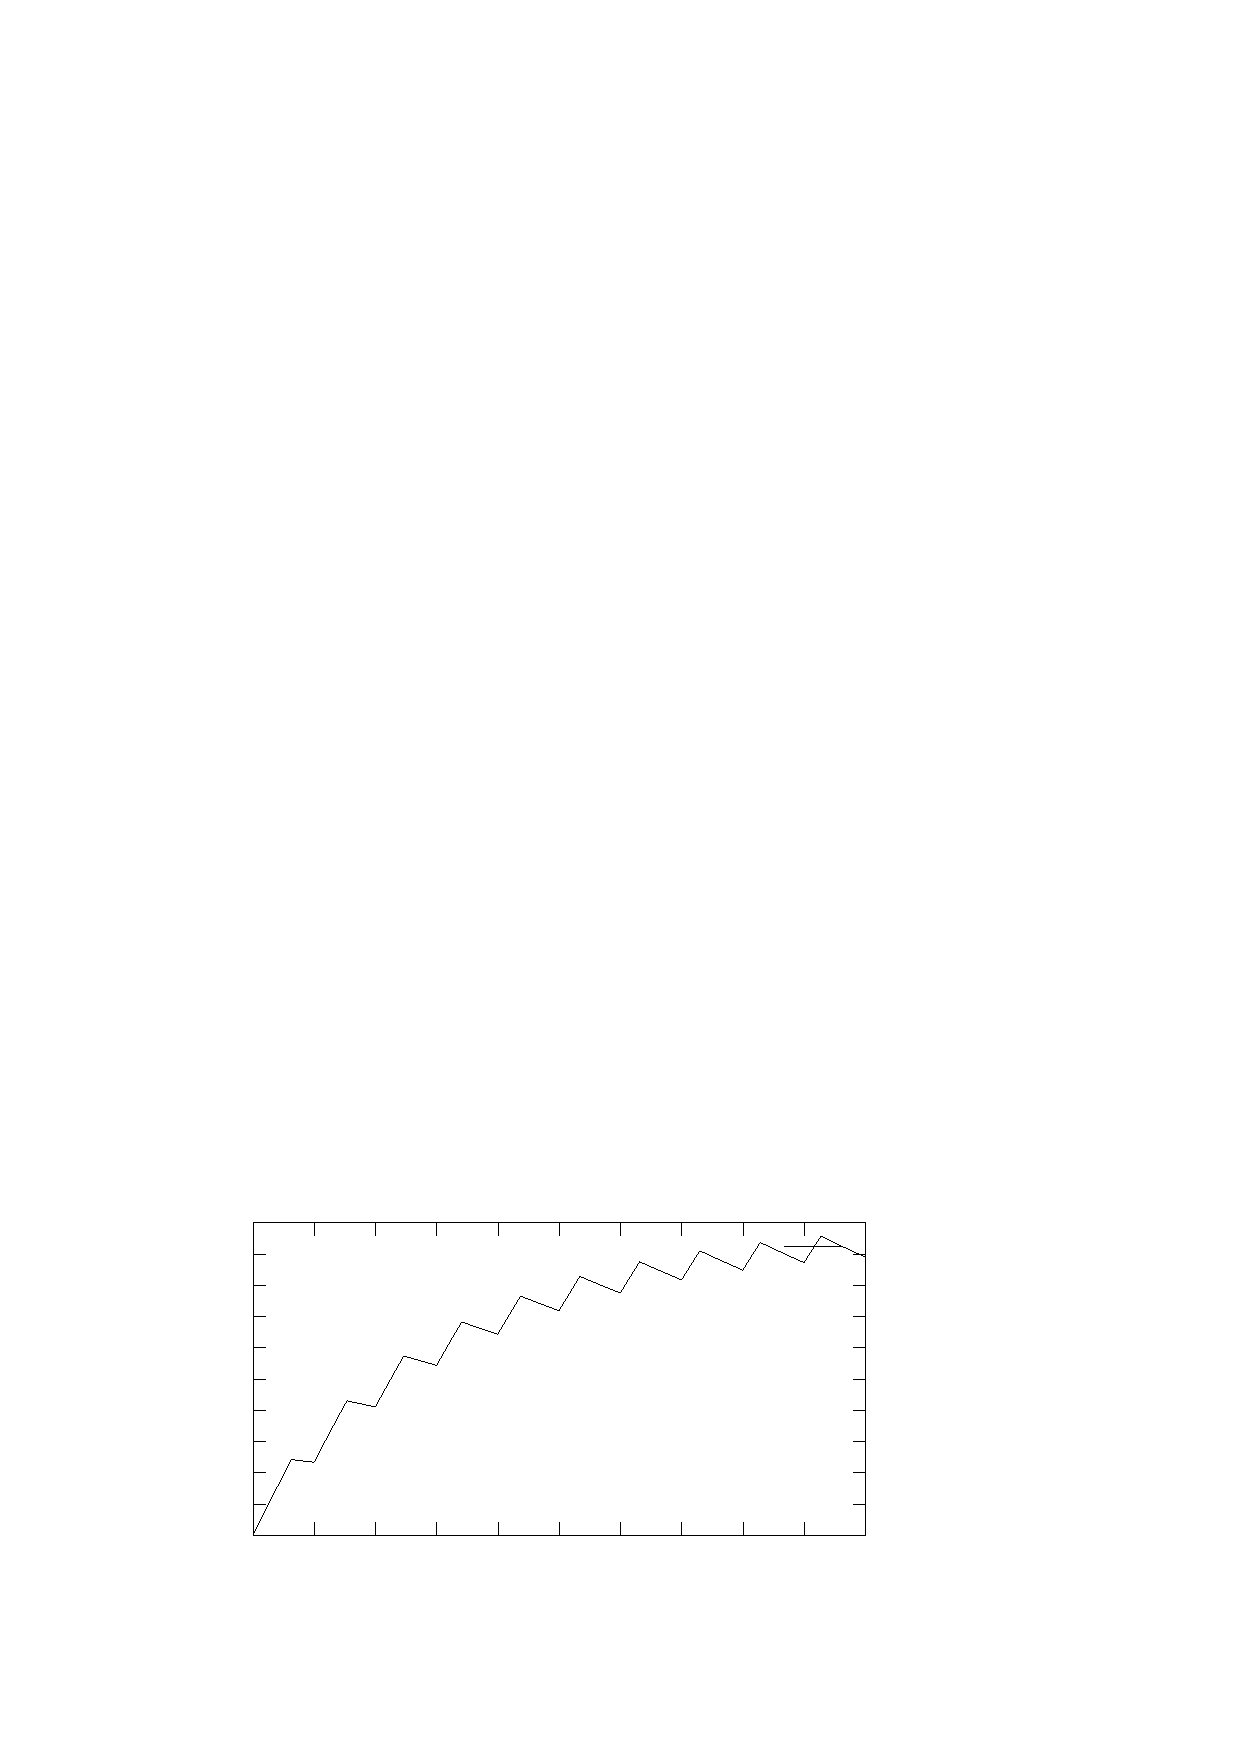
\includegraphics{CS}%
\end{picture}%
\begingroup
\setlength{\unitlength}{0.0200bp}%
\begin{picture}(18000,10800)(0,0)%
\put(2200,1650){\makebox(0,0)[r]{\strut{} 0}}%
\put(2200,2400){\makebox(0,0)[r]{\strut{} 0.5}}%
\put(2200,3150){\makebox(0,0)[r]{\strut{} 1}}%
\put(2200,3900){\makebox(0,0)[r]{\strut{} 1.5}}%
\put(2200,4650){\makebox(0,0)[r]{\strut{} 2}}%
\put(2200,5400){\makebox(0,0)[r]{\strut{} 2.5}}%
\put(2200,6150){\makebox(0,0)[r]{\strut{} 3}}%
\put(2200,6900){\makebox(0,0)[r]{\strut{} 3.5}}%
\put(2200,7650){\makebox(0,0)[r]{\strut{} 4}}%
\put(2200,8400){\makebox(0,0)[r]{\strut{} 4.5}}%
\put(2200,9150){\makebox(0,0)[r]{\strut{} 5}}%
\put(2475,1100){\makebox(0,0){\strut{} 0}}%
\put(3945,1100){\makebox(0,0){\strut{} 200}}%
\put(5415,1100){\makebox(0,0){\strut{} 400}}%
\put(6885,1100){\makebox(0,0){\strut{} 600}}%
\put(8355,1100){\makebox(0,0){\strut{} 800}}%
\put(9825,1100){\makebox(0,0){\strut{} 1000}}%
\put(11295,1100){\makebox(0,0){\strut{} 1200}}%
\put(12765,1100){\makebox(0,0){\strut{} 1400}}%
\put(14235,1100){\makebox(0,0){\strut{} 1600}}%
\put(15705,1100){\makebox(0,0){\strut{} 1800}}%
\put(17175,1100){\makebox(0,0){\strut{} 2000}}%
\put(550,5400){\rotatebox{0}{\makebox(0,0){\strut{}$I_L$}}}%
\put(9825,275){\makebox(0,0){\strut{}time ($10^{-7}s$)}}%
\put(9825,9975){\makebox(0,0){\strut{}switch circuit}}%
\end{picture}%
\endgroup
\endinput

    }
 } 
 \end{figure}



 
}

\frame
{

\frametitle{A switched circuit.}
  \begin{figure}[!h]
   \centerline{
   \scalebox{0.9}{
    \input{CSRES.pstex_t}
    }
 } 
 \end{figure}
\begin{block}{Model and equations}

\begin{equation}
\begin{array}{cc}
L \dot I_L + R_E(R_s,R_d)I_L + U_E(R_s,R_d) =0&
\frac{R_d}{R_s+R_d} (20 - R_sI_L)-V_1=0\\
R_s= \begin{cases}
R_{on} \qquad \text{if $V_3-V1 \geq 0$}\\
R_{off} \qquad \text{if $V_3-V1 < 0$}\\
\end{cases}&
R_d= \begin{cases}
R_{on} \qquad \text{if $V_1 < 0$}\\
R_{off} \qquad \text{if $V_1 \geq 0$}\\
\end{cases}
\end{array}
\end{equation}

\end{block}

 }

\frame{
\frametitle{Newton-Raphson algorithm $t_n \to t_{n+1}$}

  \begin{figure}[h]
   \centerline{
   \scalebox{0.6}{
    \input{NR_ALGO.pstex_t}
    }
 } 
 \end{figure}


}

 
 \frame
{

\frametitle{t=0, $I_L=0$}
  \begin{figure}[!h]
   \centerline{
   \scalebox{0.9}{
    \input{CST0.pstex_t}
    }
 } 
 \end{figure}
 

 \begin{block}{An linear behavior}
While the diode and the switch stay in the same state, the Newton-Raphson algorithm converges in
one iteration. It is a linear circuit.

\end{block}
 }

 \frame
{

\frametitle{t=$t_1$, the switch change of state.}

  \begin{figure}[!h]
   \centerline{
   \scalebox{0.9}{
    \input{CSTstep0.pstex_t}
    }
 } 
 \end{figure}

 \begin{block}{Newton-Raphson iterations}
\begin{equation}
\begin{array}{|c|c|c|c|c|c|c|}
\hline
&$k=0$&$k=1$&$k=2$&$k=3$&$k=4$&...\\
\hline
S&ON&&&&&\\
\hline
D&OFF&&&&&\\
\hline
\end{array}
\end{equation}
\end{block}


 }

\frame
{

\frametitle{t=$t_1$, the switch change of state.}
  \begin{figure}[!h]
   \centerline{
   \scalebox{0.9}{
    \input{CSTstep1.pstex_t}
    }
 } 
 \end{figure}
  \begin{block}{Newton-Raphson iterations}
\begin{equation}
\begin{array}{|c|c|c|c|c|c|c|}
\hline
&$k=0$&$k=1$&$k=2$&$k=3$&$k=4$&...\\
\hline
S&ON&OFF&&&&\\
\hline
D&OFF&OFF&&&&\\
\hline
\end{array}
\end{equation}
\end{block}

 }
  \frame
{

\frametitle{t:$t_1 \to t_1+h$, first Newton-Raphson iteration.}
  \begin{figure}[!h]
   \centerline{
   \scalebox{0.9}{
    \input{CSTstep2.pstex_t}
    }
 } 
 \end{figure}
  \begin{block}{Newton-Raphson iterations}
\begin{equation}
\begin{array}{|c|c|c|c|c|c|c|}
\hline
&$k=0$&$k=1$&$k=2$&$k=3$&$k=4$&...\\
\hline
S&ON&OFF&ON&&&\\
\hline
D&OFF&OFF&ON&&&\\
\hline
\end{array}
\end{equation}
\end{block}


 }
  \frame
{

\frametitle{t:$t_1 \to t_1+h$, second Newton-Raphson iteration.}
  \begin{figure}[!h]
   \centerline{
   \scalebox{0.9}{
    \input{CSTstep1.pstex_t}
    }
 } 
 \end{figure}
   \begin{block}{Newton-Raphson iterations}
\begin{equation}
\begin{array}{|c|c|c|c|c|c|c|}
\hline
&$k=0$&$k=1$&$k=2$&$k=3$&$k=4$&...\\
\hline
S&ON&OFF&ON&OFF&ON&...\\
\hline
D&OFF&OFF&ON&OFF&ON&...\\
\hline
\end{array}
\end{equation}
\end{block}

 }


\frame
{

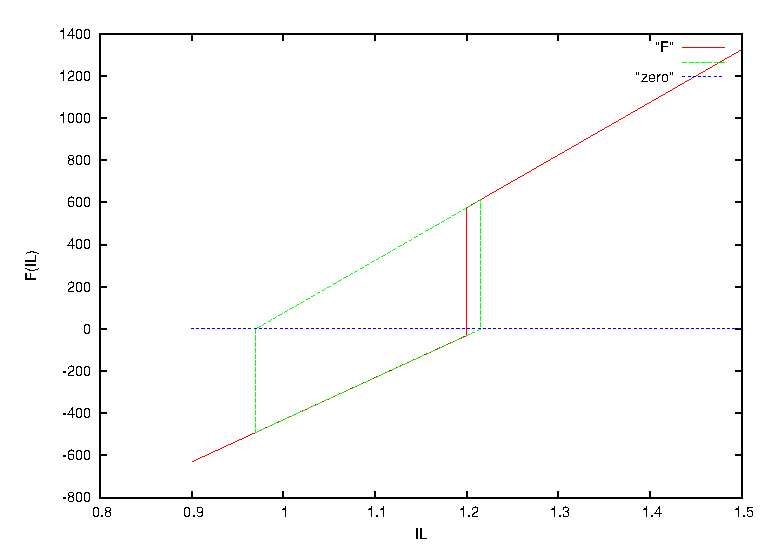
\includegraphics{F_FNR.eps}

 }
 
 \frame
{
\frametitle{Complementarity formulation.}

\begin{figure}
   \centerline{
   \scalebox{0.8}{
    \input{CSsmall.pstex_t}
    }
 } 
 \end{figure}

  
 \begin{eqnarray*}
 &{\color{Green}L\dot I_L -(V_1-V_2)=0}&V_3-e(t)=0\\
 &I_L-I_S-I_D=0&RI_L-V_2=0\\
 &{\color{Red}V_1+I_D(\lambda _4 +R_{on})}&{\color{Blue}V_1-20+I_S(\lambda _2 - R_{on})=0}\\
 &{\color{Red}y_3=R_{off}-\lambda _4 - R_{on}}&{\color{Blue}y_1=R_{off}-\lambda _2-R_{on}}\\
 &{\color{Red}y_4=-V_1+\lambda _3}&{\color{Blue}y_2=V_3-V_2+\lambda _1}\\
 \end{eqnarray*}
 \[0 \leq y_i \perp \lambda _i \geq 0\]
 }

\frame
{

\frametitle{Complementarity formulation.}
 \begin{figure}
 %GNUPLOT: LaTeX picture with Postscript
\begin{picture}(0,0)%
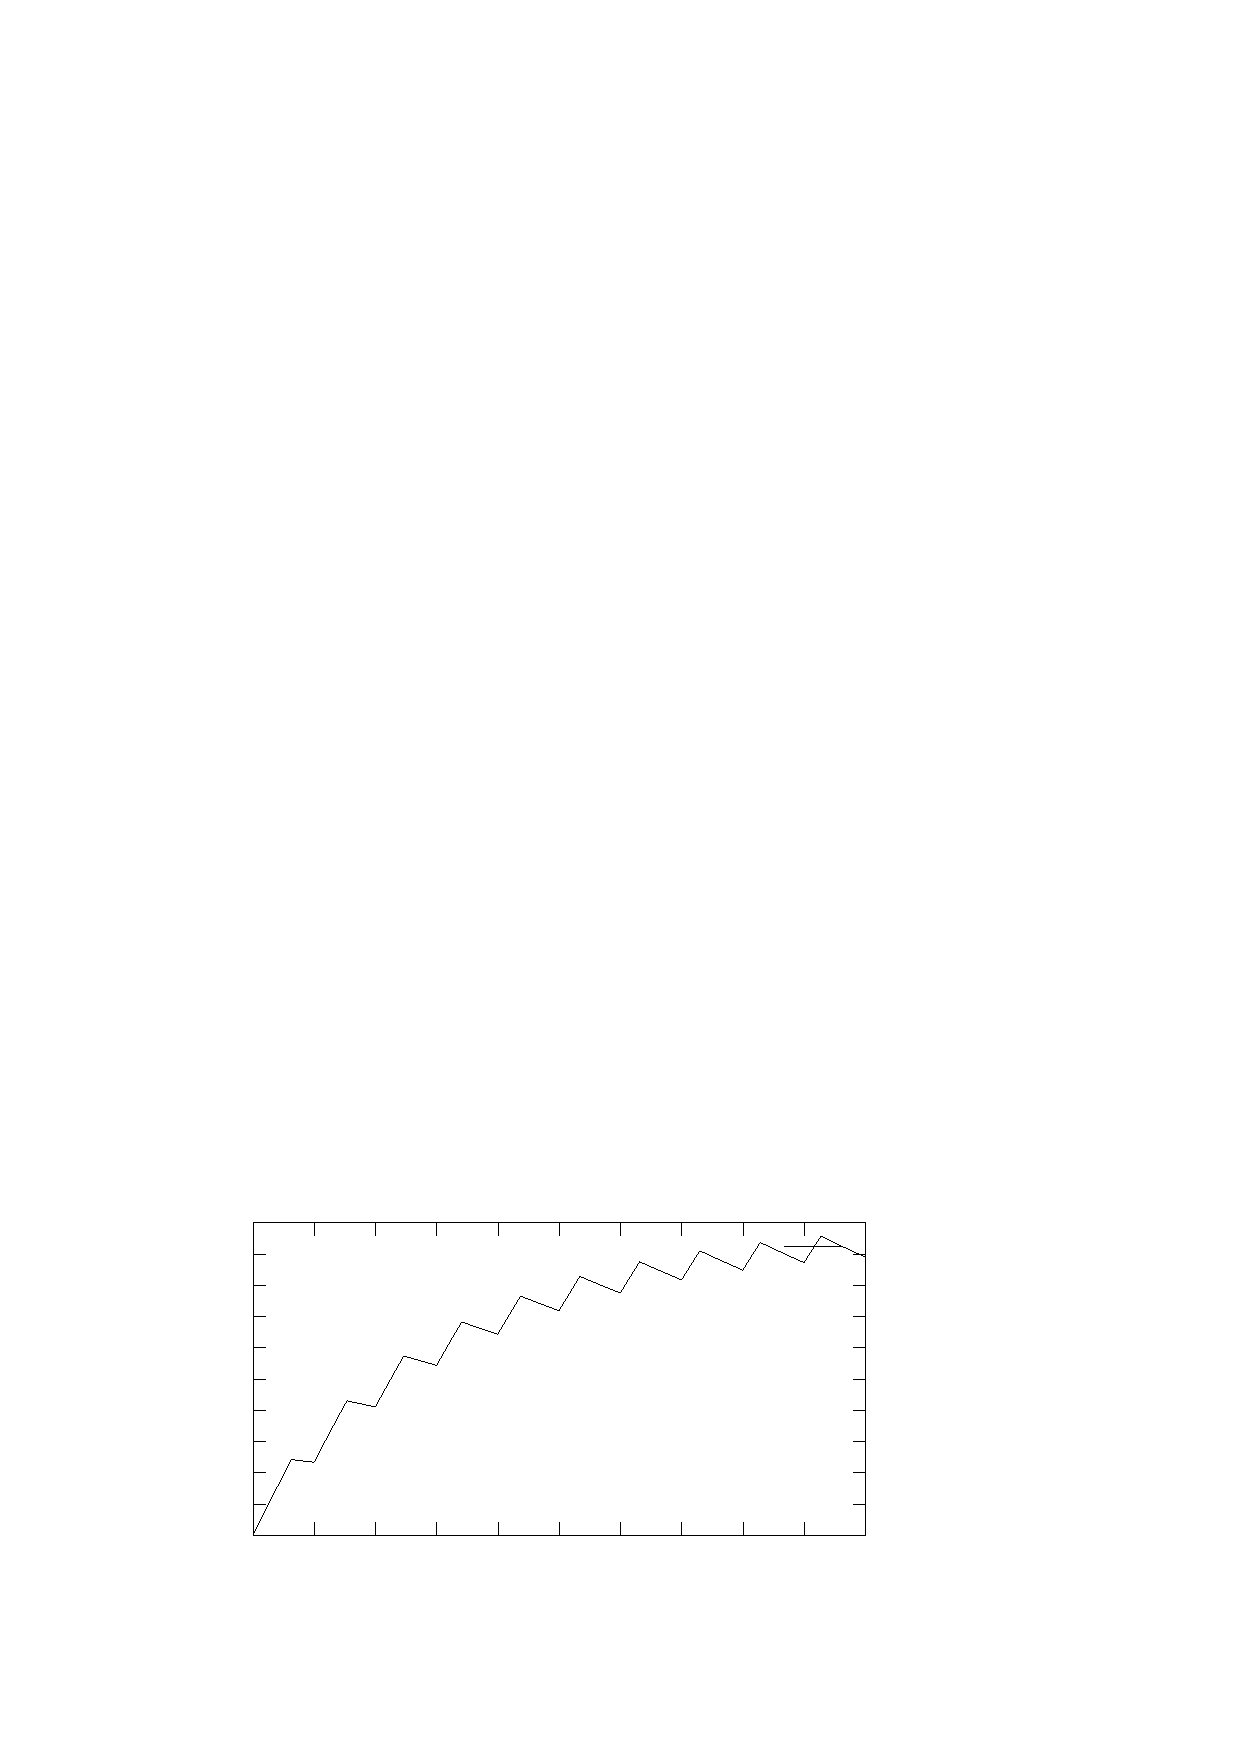
\includegraphics{CS}%
\end{picture}%
\begingroup
\setlength{\unitlength}{0.0200bp}%
\begin{picture}(18000,10800)(0,0)%
\put(2200,1650){\makebox(0,0)[r]{\strut{} 0}}%
\put(2200,2400){\makebox(0,0)[r]{\strut{} 0.5}}%
\put(2200,3150){\makebox(0,0)[r]{\strut{} 1}}%
\put(2200,3900){\makebox(0,0)[r]{\strut{} 1.5}}%
\put(2200,4650){\makebox(0,0)[r]{\strut{} 2}}%
\put(2200,5400){\makebox(0,0)[r]{\strut{} 2.5}}%
\put(2200,6150){\makebox(0,0)[r]{\strut{} 3}}%
\put(2200,6900){\makebox(0,0)[r]{\strut{} 3.5}}%
\put(2200,7650){\makebox(0,0)[r]{\strut{} 4}}%
\put(2200,8400){\makebox(0,0)[r]{\strut{} 4.5}}%
\put(2200,9150){\makebox(0,0)[r]{\strut{} 5}}%
\put(2475,1100){\makebox(0,0){\strut{} 0}}%
\put(3945,1100){\makebox(0,0){\strut{} 200}}%
\put(5415,1100){\makebox(0,0){\strut{} 400}}%
\put(6885,1100){\makebox(0,0){\strut{} 600}}%
\put(8355,1100){\makebox(0,0){\strut{} 800}}%
\put(9825,1100){\makebox(0,0){\strut{} 1000}}%
\put(11295,1100){\makebox(0,0){\strut{} 1200}}%
\put(12765,1100){\makebox(0,0){\strut{} 1400}}%
\put(14235,1100){\makebox(0,0){\strut{} 1600}}%
\put(15705,1100){\makebox(0,0){\strut{} 1800}}%
\put(17175,1100){\makebox(0,0){\strut{} 2000}}%
\put(550,5400){\rotatebox{0}{\makebox(0,0){\strut{}$I_L$}}}%
\put(9825,275){\makebox(0,0){\strut{}time ($10^{-7}s$)}}%
\put(9825,9975){\makebox(0,0){\strut{}switch circuit}}%
\end{picture}%
\endgroup
\endinput
  
 \end{figure}

 }
